This section outlines the two-stage \textit{UniRel} pipeline.
Given a query, UniRel first performs \textit{subgraph retriever} to construct and refine a task-specific subgraph via multi-stage pruning (Secs.~\ref{sec:subgraph} and~\ref{sec:prune}).
In the second stage, an RL-tuned LLM reasons over the retrieved subgraph and the query to generate an answer emphasizing the most informative relations (Sec.~\ref{sec:llm_training}). Note that the framework can be extended to alternative optimization objectives by modifying the pruning criteria and adjusting the reward function.


\begin{figure*}[t]
    \centering
    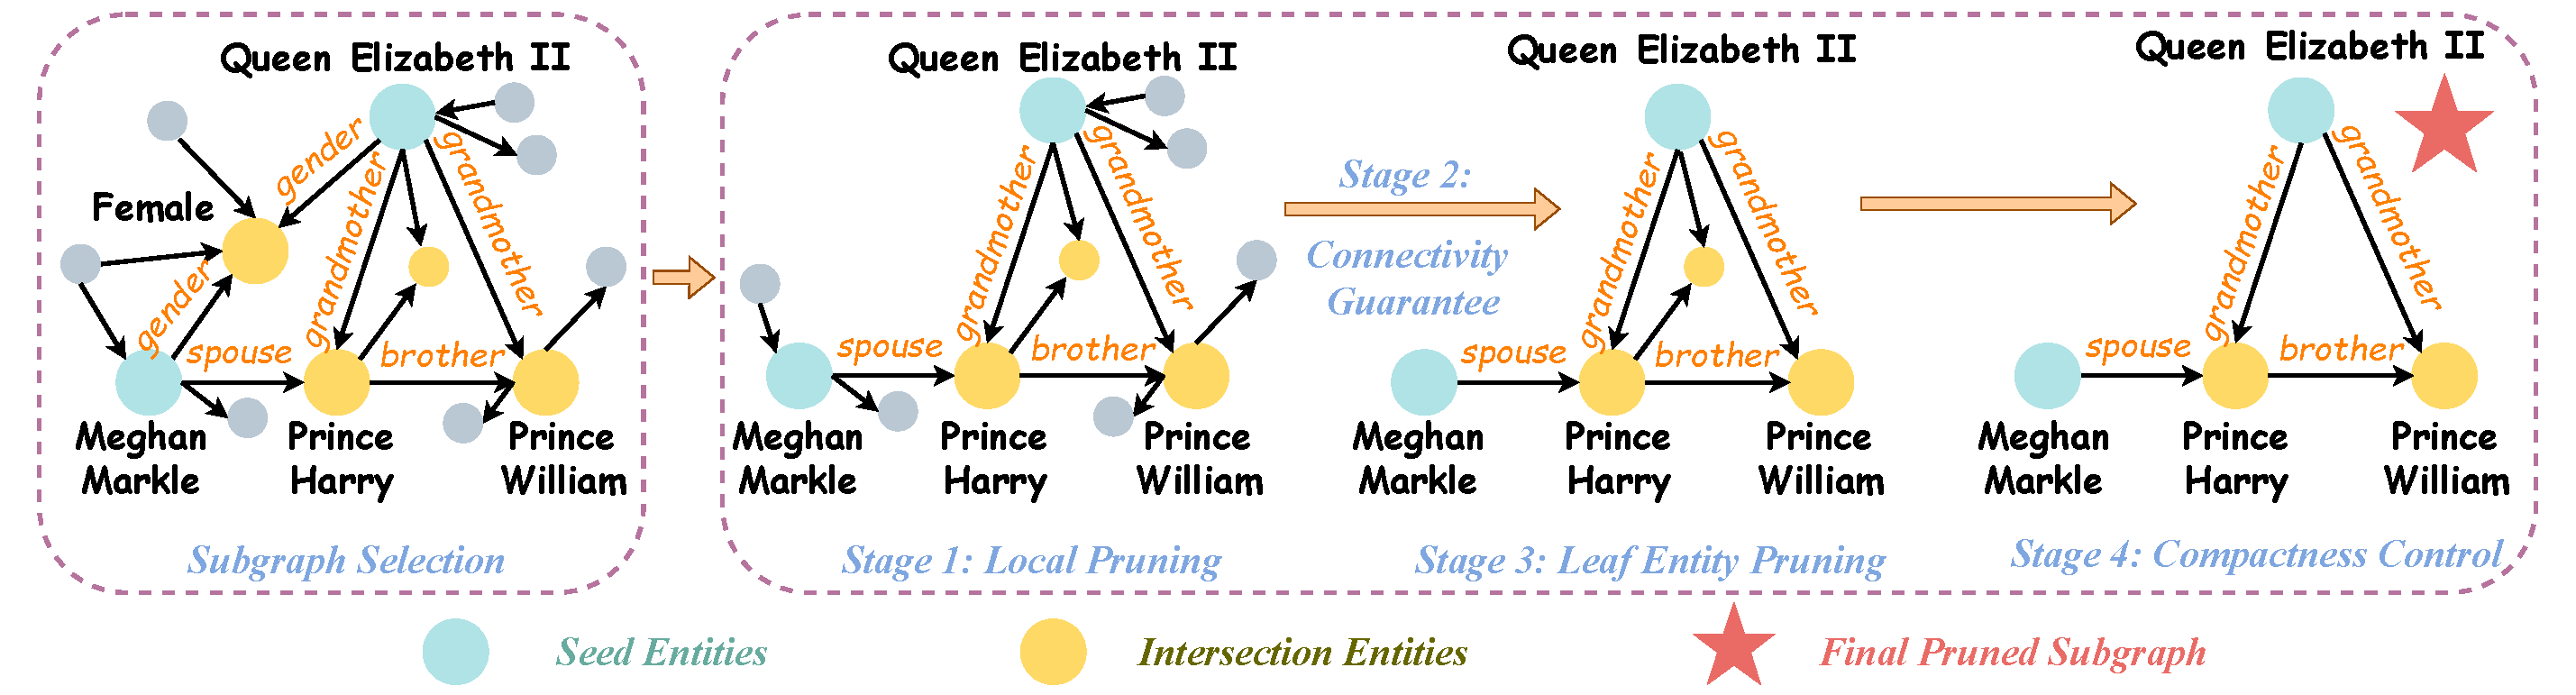
\includegraphics[width=0.86\textwidth]{figures/graph_pruning.pdf}
    \vspace{-0.5em}
    \caption{An example of multi-step graph pruning. From the initial subgraph (left), Stage~1 removes overly common entities (e.g., \textit{Female}), Stage~2 enforces connectivity through intersections, Stage~3 prunes leaf entities, and Stage~4 enhances compactness by removing high-penalty intersection nodes (yellow). The final subgraph (right) retains the most informative relations among the seed entities.}
    \vspace{-1em}
    \label{fig:graph_pruning}
\end{figure*}

% In this section, we outline the overall pipeline of \textit{UniRel-R1}, which consists of three stages.
% A task-specific subgraph is first constructed from the knowledge graph based on entities mentioned in the query (Sec.~\ref{sec:subgraph}).
% The subgraph is then refined through multi-stage pruning to remove redundant or trivial entities and relations (Sec.~\ref{sec:prune}).
% Finally, an RL-tuned LLM processes the textualized subgraph with the query to generate an answer that highlights the most informative relations(Sec.~\ref{sec:llm_training}).\footnote{Note that the framework can be extended to alternative optimization objectives by modifying the pruning criteria and adjusting the reward function accordingly.}
\subsection{Subgraph Retriever}
Subgraph retriever aims to construct a compact, task-relevant subgraph for downstream reasoning and consists of two components: subgraph selection and multi-step pruning. More details are shown in Appendix~\ref{sec:complexity}.
\subsubsection{Subgraph Selection}
\label{sec:subgraph}

Given a query $q$, the seed entity set is extracted from $q$ as $\mathcal{E}_q = \{e_1, e_2, \dots, e_m\}$.
For each seed entity $e_i \in \mathcal{E}_q$, we define its $k$-hop expansion as
{\small
$
\mathcal{V}^k(e_i) = \{ v \in \mathcal{E} \mid \mathrm{dist}(e_i,v) \leq k \},
\mathcal{T}^k(e_i) = \{ (u,r,v) \in \mathcal{T} \mid u,v \in \mathcal{V}^k(e_i) \},
$}
where $\mathrm{dist}(\cdot,\cdot)$ denotes the distance in the undirected projection of $\mathcal{G}$.


The candidate subgraph $\mathcal{G}' = (\mathcal{V}', \mathcal{R}', \mathcal{T}')$ is then obtained by aggregating the $k$-hop neighborhoods of all seed entities, where 
\small
$
\mathcal{V}' = \bigcup\nolimits_{e_i \in \mathcal{E}_q} \mathcal{V}^k(e_i), 
\mathcal{T}' = \bigcup\nolimits_{e_i \in \mathcal{E}_q} \mathcal{T}^k(e_i),
$
\normalsize
and
\small
$
\mathcal{R}' = \{ r \in \mathcal{R} \mid (u,r,v) \in \mathcal{T}' \}.
$
\normalsize
The subgraph $\mathcal{G}'$ serves as the initial candidate, refined through pruning in the next stage.





\subsubsection{Multi-step Graph Pruning}
\label{sec:prune}
The candidate subgraph $\mathcal{G}' = (\mathcal{V}', \mathcal{R}', \mathcal{T}')$  
often contains redundant structures and overly generic entities that obscure meaningful relational patterns.  
To mitigate this issue, we refine $\mathcal{G}'$ through a principled multi-stage pruning process.  

As a measure of entity generality, we introduce the \textit{hub penalty}, defined for each $e \in \mathcal{E}$ as:
{\small
\begin{equation}\label{eq:hub_penalty}
    \mathrm{HubPenalty}(e) = \log \big( 1 + \deg(e) \big),
\end{equation}
}
where $\deg(e)$ denotes the degree of $e$ in the undirected projection of $\mathcal{G}$.  
The penalty increases with entity degree, such that highly connected entities (e.g., \textit{male}) 
receive larger values, while rarer and more specific entities (e.g., \textit{president}) are penalized less.
This formulation provides a principled criterion for filtering out uninformative entities and guiding the pruning of $\mathcal{G}'$.



Figure~\ref{fig:graph_pruning} shows the multi-stage pruning on the example in Figure~\ref{fig:overview}, with each stage explained below.
% \paragraph{Stage 1: Local Pruning.}  

\textbf{Stage 1: Local Pruning.}
For each expansion set $\mathcal{V}^k(e_i)$, we impose a threshold $\rho$ on the hub penalty to eliminate overly common entities.    
Each \textbf{non-seed}  $v$ with $\mathrm{HubPenalty}(v) \geq \rho$ is removed along with its incident relations.  
Subsequently, entities that become isolated (i.e., with no incident relations) are discarded.  
The resulting pruned neighborhoods are denoted by $\mathcal{V}_\rho^k(e_i)$ and $\mathcal{T}_\rho^k(e_i)$.
% \paragraph{Stage 2: Connectivity Guarantee.} 

\textbf{Stage 2: Connectivity Guarantee.}
Following local pruning, the filtered neighborhoods $\{\mathcal{V}_\rho^k(e_i)\}$ may fail to ensure connectivity among all seed entities.  
To evaluate connectivity, we compute pairwise intersections 
\small
$\mathcal{I}_{ij} = \mathcal{V}_\rho^k(e_i) \cap \mathcal{V}_\rho^k(e_j)$ 
\normalsize
and construct an auxiliary graph
\small
$
\mathcal{H}_\rho = ( \{ \mathcal{V}_\rho^k(e_i) \}, \; \{ (i,j) \mid \mathcal{I}_{ij}\neq \emptyset \} ),
$
\normalsize
where each node represents a pruned neighborhood $\mathcal{V}_\rho^k(e_i)$,  
and an edge $(i,j)$ is introduced whenever their intersection is non-empty.  
If $\mathcal{H}_\rho$ is connected, then all seed entities are jointly connected in the candidate subgraph.  
Otherwise, $\rho$ is incrementally relaxed and Stages~1--2 are repeated until graph $\mathcal G_\rho = (\mathcal{V}_{\rho}, \mathcal{R}_{\rho}, \mathcal{T}_{\rho})$ becomes connected.


% Otherwise, the threshold $\rho$ is incrementally relaxed and Stage~1 is reapplied until connectivity is restored.
% Otherwise, the threshold $\rho$ is incrementally relaxed, and Stages~1--2 are reapplied to obtain an updated subgraph $\mathcal G'_\rho$ until connectivity is restored.

\textbf{Stage 3: Leaf Entity Pruning.}
% \paragraph{Stage 3: Leaf Entity Pruning.}  
Once connectivity is ensured, we iteratively eliminate non-seed entities in  $\mathcal G_\rho$ whose neighbor set \small $\mathcal{N}_{\rho}(v) = \{ u \in \mathcal{V}_{\rho} \mid \exists r \in \mathcal{R}_{\rho}: (v,r,u) \in \mathcal{T}_{\rho}$ or $(u,r,v) \in \mathcal{T}_{\rho} \}$ \normalsize contains only a single distinct element (\small $|\mathcal{N}_{\rho}(v)| = 1$\normalsize). Such leaf-like entities and their incident relations are iteratively pruned until no removal is possible. 

% Once connectivity is ensured, we iteratively remove non-seed entities in $\mathcal G_\rho$ whose neighbor set
% \[
% \mathcal N(v) = \{ u \in \mathcal V_\rho \mid \exists r \in \mathcal R_\rho : (v,r,u) \in \mathcal T_\rho \ \text{or}\ (u,r,v) \in \mathcal T_\rho \}
% \]
% contains only a single distinct element, i.e., $|\mathcal N(v)| = 1$.

\textbf{Stage 4: Compactness Control.}
% \paragraph{Stage 4: Compactness Control.} 
If the refined subgraph remains large $\mathcal G'_\rho$, we further enforce compactness by leveraging the intersections \small $\{\mathcal{I}_{ij}\}$ \normalsize defined in Stage~2.  
Let \small $\mathcal{I}^+ = \{\mathcal{I}_{ij} \mid \mathcal{I}_{ij} \neq \emptyset\}$ \normalsize denote the collection of all non-empty intersections.  
We then select a subset \small $\mathcal{I}^c \subseteq \mathcal{I}^+$ \normalsize whose index pairs jointly cover all seed entities, i.e.,
\small
$
\bigcup\nolimits_{\mathcal{I}_{ij} \in \mathcal{I}^c} \{i,j\} = \{0,1,\dots,m-1\}.
$
\normalsize
For each valid subset $\mathcal{I}^c$, a candidate subgraph is constructed in two steps.  
First, within each intersection $\mathcal{I}_{ij}$, we retain $s$ entities with lowest hub penalties:
$$
\widehat{\mathcal{I}}_{ij} 
= \argmin\nolimits_{\substack{\mathcal{U} \subseteq \mathcal{I}_{ij}, |\mathcal{U}| = s}} 
\sum\nolimits_{v \in \mathcal{U}} \mathrm{HubPenalty}(v).
$$
Second, each selected set $\widehat{\mathcal{I}}_{ij}$ is expanded via a $k$-hop search restricted to the corresponding pruned neighborhoods:
\small
$
\mathcal{N}^k(\widehat{\mathcal{I}}_{ij}) 
= \widehat{\mathcal{I}}_{ij} \cup \{ u \in \mathcal{V}_\rho^k(e_i) \cup \mathcal{V}_\rho^k(e_j) \mid \mathrm{dist}(u,v) \leq k ,\ v \in \widehat{\mathcal{I}}_{ij} \}.
$
\normalsize
The candidate node set associated with $\mathcal{I}^c$ is then
\small $\mathcal{V}(\mathcal{I}^c) = \bigcup_{\mathcal{I}_{ij} \in \mathcal{I}^c} \mathcal{N}^k(\widehat{\mathcal{I}}_{ij})$\normalsize,
and its induced subgraph is subsequently simplified using Stage~3.  

Finally, the most compact subgraph under parameters $(s,\rho)$ is obtained as:
\small
\[
\mathcal{G}^{s}_{\rho} = (\mathcal{V}^{s}_{\rho}, \mathcal{R}^{s}_{\rho}, \mathcal{T}^{s}_{\rho}),
\]
\normalsize
where \small $\mathcal{V}^{s}_{\rho} = \argmin_{\mathcal{S} \in \mathcal{I}^+} \; |\mathcal{V}(\mathcal{S})|$, $\mathcal{T}^{s}_{\rho} \!= \!\{ (u,r,v) \in \mathcal{T}'_{\rho} \mid u,v \in \mathcal{V}^{m}_{\rho} \}$, \small $\mathcal{R}^{s}_{\rho} = \{ r \in \mathcal{R}'_{\rho} \mid (u,r,v) \in \mathcal{T}^{s}_{\rho} \}$\normalsize.

\textbf{Stage 5: Iterative Reduction.}
% \paragraph{Stage 5: Iterative Reduction.}   
If the subgraph still exceeds the target size, we decrease $s$ and reapply Stage~4
until a sufficiently compact subgraph is obtained.



\subsection{Relational Answer Generation via LLM}
\label{sec:llm_training}
Given the refined subgraph $\mathcal{G}^{m}_{\rho}$, the final step is to generate an answer that highlights the most informative relational structure.  
We employ an RL-tuned LLM to produce relational explanations conditioned on the query and textualized subgraph,
optimized using task-specific rewards detailed in the following sections.


\subsubsection{Reinforcement Learning Algorithms}
\textbf{RL with Verifiable Reward (RLVR).}
Our approach builds on the RLVR paradigm~\citep{Lambert2024TLU3P}, which applies to settings where response quality can be deterministically verified.
In its standard form, RLVR uses a rule-based verifier $v : \mathcal{X} \to \{0,1\}$ to assign binary rewards: $r_i = v(x_i)$, where $v(x_i)=1$ if $x_i$ passes a task-specific correctness check, and $0$ otherwise.
This binary scheme is effective for tasks with unambiguous success criteria (e.g., mathematical problem-solving and code generation).  
In our setting, we design a corresponding rule-based reward to verify model generated relations, described in Sec.~\ref{sec:reward}.


\textbf{Group Relative Policy Optimization (GRPO).}
For policy optimization, we adopt GRPO~\citep{shao2024deepseekmath},  
which evaluates responses based on their relative performance within a sampled group from the policy.  

Given a query $q$, we sample from the previous policy $\pi_{\theta_{\mathrm{old}}}(\cdot\!\mid q)$ to get $G$ responses $\{o_i\}_{i=1}^G$ with rewards $\{r_i\}$.
The advantage $A_i$ is the group-normalized reward, defined as:
\small
$$
A_i = \frac{r_i - \overline{r}}
     {\sqrt{\tfrac{1}{G}\sum_{j=1}^G (r_j - \overline{r})^2} + \varepsilon_{\mathrm{stab}}}, \quad \overline{r} = \frac{1}{G}\sum_{j=1}^G r_j,
$$
\normalsize
where $\varepsilon_{\mathrm{stab}}$ ensures numerical stability. 
With $\rho_i=\frac{\pi_{\theta}(o_i\!\mid q)}{\pi_{\theta_{\mathrm{old}}}(o_i\!\mid q)}$,
% the GRPO objective maximizes a clipped surrogate similar to PPO:
GRPO loss is defined as a clipped surrogate similar to PPO:
% ~\jh{I feel that you can use J as the symbol for training objective (as the one used in GRPO paper) instead of L, which means loss function (which needs a negative sign here).}
\small \begin{equation*}
\begin{aligned}
    \mathcal{L}_{\mathrm{GRPO}}(\theta)
 =&
-
[
\frac{1}{G}\sum_{i=1}^G
\min\!\bigl(\rho_i A_i,\;\!\!\mathrm{clip}(\rho_i,1-\alpha,1+\alpha)\,A_i\bigr) \\
& -\;\!\!\beta\,D_{\mathrm{KL}}\bigl(\pi_{\theta}(\cdot|q)\,\Vert\,\pi_{\mathrm{ref}}(\cdot|q)\bigr)
].
\end{aligned}    
\end{equation*}
\normalsize
This objective encourages policy $\pi_{\theta}$ to favor above-average responses.
A $\beta$-scaled KL term regularizes updates to limit deviations from the reference policy $\pi_{\mathrm{ref}}$.


% For policy optimization, we employ Group Relative Policy Optimization (GRPO)~\citep{shao2024deepseekmath}. The core idea is to evaluate responses based on their performance relative to a group of candidates sampled from the policy.

% Given a prompt $q$, we sample $G$ responses $\{o_i\}_{i=1}^G$ from the frozen policy $\pi_{\theta_{\mathrm{old}}}(\cdot\!\mid q)$, with corresponding rewards $\{r_i\}$. The advantage $A_i$ for each response is its standardized reward, normalized by the group's mean and standard deviation. Let $\rho_i = \frac{\pi_{\theta}(o_i\!\mid q)}{\pi_{\theta_{\mathrm{old}}}(o_i\!\mid q)}$ be the importance sampling ratio. The advantage is defined as:
% $$
% \overline{r} = \frac{1}{G}\sum_{j=1}^G r_j,
% \qquad
% A_i = \frac{r_i - \overline{r}}
%      {\sqrt{\tfrac{1}{G}\sum_{j=1}^G (r_j - \overline{r})^2} + \varepsilon_{\mathrm{stab}}},
% $$
% where $\varepsilon_{\mathrm{stab}}$ is a small constant for numerical stability. The GRPO objective, which we aim to maximize, is a clipped surrogate objective similar to PPO:
% $$
% \mathcal{L}_{\mathrm{GRPO}}(\theta)
% =
% \mathbb{E}_{\substack{q\sim\mathcal{D}\\\{o_i\}\sim\pi_{\theta_{\mathrm{old}}}}}
% \Biggl[
% \frac{1}{G}\sum_{i=1}^G
% \min\!\bigl(\rho_i A_i,\;\!\!\mathrm{clip}(\rho_i,1-\alpha,1+\alpha)\,A_i\bigr)\!\!
% \;-\;\!\!\beta\,D_{\mathrm{KL}}\bigl(\pi_{\theta}(\cdot|q)\,\Vert\,\pi_{\mathrm{ref}}(\cdot|q)\bigr)
% \Biggr].
% $$
% This objective encourages the policy $\pi_{\theta}$ to assign higher probabilities to responses with above-average rewards within the sampled group. The KL divergence term, weighted by $\beta$, regularizes the policy updates to prevent large deviations from a reference policy $\pi_{\mathrm{ref}}$.


% Our approach is based on the RLVR paradigm~\citep{Lambert2024TLU3P}. This framework is designed for domains where the quality of a generated response can be deterministically and automatically verified. In its standard form, RLVR employs a rule-based verifier $v : \mathcal{X} \to \{0,1\}$ that assigns a simple binary reward to each generation $x_i$:
% \[
%  r_i \;=\; v(x_i)
%  \;=\;
%  \begin{cases}
%    1, & \text{if } x_i \text{ satisfies a task-specific correctness check},\\[4pt]
%    0, & \text{otherwise}.
%  \end{cases}
% \]
% This binary reward structure is highly effective for tasks with unambiguous success criteria, such as mathematical problem-solving and code generation. For our task, we design a corresponding rule-based reward, which is detailed in Section~\ref{sec:reward}.
\normalsize
\subsubsection{Reward design}
\label{sec:reward}

In relation-centric KGQA, a valid answer must follow the format, ensure connectivity, and emphasize informative entities and relations.  
To capture these aspects, we design a composite reward with four components: \emph{Format}, \emph{Connectivity}, \emph{Entity Informativeness}, and \emph{Relation Informativeness}.


Formally, for each answer $a$, we define:

\textbf{Format Reward.} The format reward is defined as $R_{\mathrm{fmt}}(a) \in \{-1,1\}$, where $R_{\mathrm{fmt}}(a) = 1$ when $a$ conforms to the required format and $R_{\mathrm{fmt}}(a) = -1$ otherwise.

\textbf{Connectivity Reward.}
% \paragraph{Connectivity Reward.} 
The connectivity reward evaluates whether the output subgraph connects the extracted entities $\mathcal{E}_q$ and is defined as $R_{\mathrm{con}}(a) \in \{-\lfloor |\mathcal{E}_q|/2 \rfloor, \dots, \lceil |\mathcal{E}_q|/2 \rceil - 1\}$, where the minimum indicates full disconnection, intermediate values reflect partial connectivity (e.g., $-\lfloor |\mathcal{E}_q|/2 \rfloor + l$ for $(l+1)$-connected entities), and the maximum denotes full connectivity.


% The connectivity reward evaluates whether the output subgraph connects the extracted entities $\mathcal{E}_q$, with the following cases:  
% \squishlist
%  \item $|\mathcal{E}_q| = 2$: $R_{\mathrm{rch}}(a) \in \{-1,0\}$, taking value $0$ if the two entities are connected and $-1$ otherwise. 
%   \item$|\mathcal{E}_q| > 2$: $R_{\mathrm{rch}}(a) \in \{-\lceil |\mathcal{E}_q|/2 \rceil + 1, \dots, \lfloor |\mathcal{E}_q|/2 \rfloor\}$, where the minimum indicates full disconnection, intermediate values reflect partial connectivity (e.g., $-\lceil |\mathcal{E}_q|/2 \rceil + k$ for $k$-connected entities), and the maximum denotes full connectivity.
% \squishend

\textbf{Entity Informativeness Reward.} 
This component favors informative over generic entities.  
For a generated answer $a$ with entity set $\mathcal{E}(a)$,  
the reward is the sum of normalized hub penalties:
\vspace{-1em}
\small
\begin{equation}\label{eq:entity_informativenss}
R_{\mathrm{ent}}(a) = \!\!\!\!\sum_{e \in \mathcal{E}(a)} \!\!\!R_{\mathrm{ent}}(e), R_{\mathrm{ent}}(e) \!= \!\!- \frac{\mathrm{HubPenalty}(e)}{\max_{v \in \mathcal{E}} \mathrm{HubPenalty}(v)},
\end{equation}
\normalsize
where $\mathrm{HubPenalty}(e)$ is defined in Equation~\ref{eq:hub_penalty}.

\textbf{Relation Informativeness Reward.} This component favors infrequent relations, which are more informative.
The informativeness of a relation $r$ is measured by its inverse document frequency (IDF)~\citep{robertson2004understanding}:
\small
$
\mathrm{IDF}(r) = \log \!\left(\frac{|\mathcal{T}|}{|\{(u,r,v)\in \mathcal{T}\}|}\right),
$
\normalsize
where $|\mathcal{T}|$ is the number of triples in $\mathcal{G}$ and the denominator is the frequency of $r$.  
Frequent relations (e.g., \textit{gender}) receive lower IDF scores, while rarer ones (e.g., \textit{invention}) score higher. 

Given an answer $a$ with relation set $\mathcal{R}(a)$, the reward is the sum of normalized IDF scores:
\small
\begin{equation}\label{eq:relation_informativenss}
\vspace{-1em}
R_{\mathrm{rel}}(a) = \sum_{r \in \mathcal{R}(a)} R_{\mathrm{rel}}(r),
R_{\mathrm{rel}}(r) = \frac{\mathrm{IDF}(r)}{\max\nolimits_{s \in \mathcal{R}} \mathrm{IDF}(s)} - 1.
\end{equation}
\normalsize


\textbf{Overall Reward.}  
The final reward for an answer $a$ aggregates all four components:
\small
\begin{equation}\label{eq:reward}
    R(a) = R_{\mathrm{fmt}}(a) 
+ R_{\mathrm{con}}(a) 
+ \tfrac{1}{2}\!\left(\tfrac{R_{\mathrm{ent}}(a)}{x} 
+ \tfrac{R_{\mathrm{rel}}(a)}{y}\right),
\end{equation}
\normalsize
where $x$ and $y$ are normalization constants ensuring  
$\tfrac{R_{\mathrm{ent}}(a)}{x}, \tfrac{R_{\mathrm{rel}}(a)}{y} \in [-1,0]$,  
with values determined by the maximum permitted subgraph size.  

By construction, the reward is bounded as a function of the number of seed entities $|\mathcal{E}_q|$: $R(a) \in [-\lfloor |\mathcal{E}_q|/2 \rfloor- 2, \lceil |\mathcal{E}_q|/2 \rceil)$.
If $R_{\mathrm{fmt}}(a)=-1$, then $R(a)=-\lfloor |\mathcal{E}_q|/2 \rfloor- 2$.  
If $R_{\mathrm{con}}(a)=-\lfloor |\mathcal{E}_q|/2 \rfloor$,  
then $R(a)=-\lfloor |\mathcal{E}_q|/2 \rfloor$.

% \small
% \[
% R(a) \in 
% \begin{cases}
% [-3,\,1), & \text{if } |\mathcal{E}_q| = 2, \\[6pt]
% \bigl[-\lceil |\mathcal{E}_q|/2 \rceil - 1,\;\lfloor |\mathcal{E}_q|/2 \rfloor + 1\bigr), & \text{if } |\mathcal{E}_q| > 2.
% \end{cases}
% \]
% \normalsize
% Let $R_{\min}(|\mathcal{E}_q|)$ denote the lower bound.  
% If $R_{\mathrm{fmt}}(a)=-1$, then $R(a)=R_{\min}(|\mathcal{E}_q|)$.  
% If $R_{\mathrm{con}}(a)=-\lceil |\mathcal{E}_q|/2 \rceil+1$,  
% then $R(a)=R_{\min}(|\mathcal{E}_q|)+2$.

